\documentclass[../notes.tex]{subfiles}

\pagestyle{main}
\renewcommand{\chaptermark}[1]{\markboth{\chaptername\ \thechapter\ (#1)}{}}
\setcounter{chapter}{3}

\begin{document}




\chapter{Normal Subgroups: Motivation and Properties}
\section{Quotient Groups}
\begin{itemize}
    \item \marginnote{10/17:}Notational confusion regarding $\Z/10\Z$.
    \begin{itemize}
        \item Let $G=\Z$ and $H=10\Z$ (the multiples of 10).
        \item A few of the cosets are as follows:
        \begin{align*}
            H &= \{\dots,-20,-10,0,10,20,30,\dots\}\\
            1+H &= \{\dots,-19,-9,1,11,21,31,\dots\}\\
            2+H &= \{\dots,-18,-8,2,12,22,32,\dots\}
        \end{align*}
        \item Evidently, $|\Z/10\Z|=10$.
        \item Yet $\Z/10\Z$ is also the notation for the cyclic group of order 10.
        \item This notation is not an error, but reveals something deep: We can make the set of cosets into a group and define addition by
        \begin{equation*}
            (a+10\Z)+(b+10\Z) = (a+b+10\Z)
        \end{equation*}
        More specifically, we can define an isomorphism between the two definitions of $\Z/10\Z$ via $a+H\mapsto a$ for $a=0,\dots,9$.
    \end{itemize}
    \item This example motivates the following goal.
    \item Goal: Make $G/H$, which is a set, into a group.
    \begin{itemize}
        \item This set needs a binary operation. It makes natural sense to define the binary operation as follows.
        \begin{equation*}
            xH*yH = xyH
        \end{equation*}
        \item We then need an identity coset, inverse cosets, and associativity.
        \begin{itemize}
            \item The identity is $H$.
            \item The inverse of $xH$ is $x^{-1}H$.
            \item Associativity of $G/H$ follows from the associativity of $G$ (which tells us that $(ab)c=a(bc)$). More specifically,
            \begin{align*}
                aH*_H(bH*_HcH) &= aH*_H(b*_Gc)H\\
                &= a*_G(b*_Gc)H\\
                &= (a*_Gb)*_gcH\\
                &= (a*_Gb)H*_HcH\\
                &= (aH*_HbH)*_HcH
            \end{align*}
        \end{itemize}
    \end{itemize}
    \item Calegari's impromptu explanation of associativity drives home that he really is very good at drilling down to the core of an idea and working with it. He really has a very similar mind to mine.
    \item Something else we need to investigate: Equivalence classes, and defining functions on equivalence classes.
    \begin{itemize}
        \item We need to make sure that functions are defined the same regardless of how you label the equivalence classes.
        \item Consider the set of names.
        \begin{itemize}
            \item Say we define equivalency classes based on all names which share the same first letter.
            \item Then we define a function $F$ on the equivalency classes based on the last letter.
            \item But then $[\text{Frank}]=[\text{Fen}]$ will be mapped to two different elements of the alphabet, so $F$ is not well-defined.
        \end{itemize}
        \item Thus, for our example, we need to guarantee that if $x,x'\in xH$, then $xH*yH=x'H*yH$.
    \end{itemize}
    \item Check: Independence of choice.
    \begin{itemize}
        \item Suppose we relabel $x\mapsto xh$ and $y\mapsto yh$. We need
        \begin{equation*}
            xhyh' = xyh''
        \end{equation*}
        for some $h''\in H$.
        \begin{itemize}
            \item Note that $x,y,h,h'$ are all fixed; $h''$ is the only free thing (i.e., is what we're looking for).
        \end{itemize}
        \item Algebraically manipulating the above implies that we want
        \begin{align*}
            h'' &= y^{-1}hyh'
        \end{align*}
        \item Thus, we know that $h''\in G$, but we need to make sure that $h''\in H$. Alternatively, we want $y^{-1}hy=h''(h')^{-1}\in H$.
        \item An example where $y^{-1}hy$ is not in $H$: $G=S_3$, $H=\gen{(1,2)}$, $h=(1,2)$, $y=(1,3)$, $yhy^{-1}=(2,3)$.
    \end{itemize}
    \item Why did $\Z/10\Z$ work? Because it was abelian, so conjugacy cancelled $y^{-1}hy=y^{-1}yh=h$.
    \begin{itemize}
        \item We could restrict ourselves entirely to abelian groups, but can we be more general?
    \end{itemize}
    \item What should we require of $G/H$?
    \begin{itemize}
        \item The cananonical map of sets $\phi:G\to G/H$ is given by $\phi(x)=xH$.
        \item We should require that $\phi$ is a homomorphism (i.e., that the group structure of $G$ is preserved for $G/H$).
        \item See how $xH*yH=xyH$ is analogous to $\phi(x)\phi(y)=\phi(xy)$.
    \end{itemize}
    \item Let's suppose $\phi:G\to G/H$ is a homomorphism.
    \begin{itemize}
        \item Then $\phi(g)=eH$ implies that $g\in H$, i.e., $\ker\phi=H$.
        \item Realization: An alternate way to do HW3, Q2b would have been in terms of quotient groups: In that case, $G/H\cong S_{26}$, and the following proposition would give us the surjectivity and kernel requirements.
    \end{itemize}
    \item Lemma: Let $\phi$ be a homomorphism from $G$ to another group. Let $K=\ker\phi\subset G$. Then $K$ has the following property, which is not true for all subgroups but is for kernels: If $x\in K$ and $g\in G$, then $gxg^{-1}\in K$.
    \begin{proof}
        Since $\phi(x)=e$, we have that
        \begin{equation*}
            \phi(gxg^{-1}) = \phi(g)\phi(x)\phi(g^{-1})
            = \phi(g)\phi(g^{-1})
            = e
        \end{equation*}
    \end{proof}
    \item \textbf{Normal} (subgroup): A subgroup $H$ of $G$ such that for all $x\in H$ and $g\in G$, $gxg^{-1}\in H$. \emph{Denoted by} $\bm{H\trianglelefteq G}$, $\bm{H\triangleleft G}$.
    \begin{itemize}
        \item We often write $gHg^{-1}$.
    \end{itemize}
    \item Example: As per the lemma, $\ker\phi$ is a normal subgroup.
    \item Example: If $G$ be abelian, then every $H\trianglelefteq G$.
    \item Lemma: A subset $H\subset G$ is normal iff
    \begin{enumerate}
        \item $H$ is a subgroup.
        \item $H$ is a union of some number of conjugacy classes.
    \end{enumerate}
    \item Proposition: Let $G$ be a group and $H\triangleleft G$. Then $G/H$ is a group under the multiplication
    \begin{equation*}
        xH*yH = xyH
    \end{equation*}
    and the map $\phi:G\to G/H$ is a surjective homomorphism with kernel $H$.
    \begin{proof}
        We want to show that $xhyh'=xyh''h'$. We can do so via multiplying the following by $x$ on the left and $h'$ on the right:
        \begin{align*}
            hy &= (yy^{-1})hy\\
            &= y(y^{-1}hy)\\
            &= yh''
        \end{align*}
        Note that we get from the second to the third line above because $H$ is a normal subgroup, i.e., conjugates of its elements are elements of it. This implies the desired result.
    \end{proof}
    \item Example: Let $G=\Z$, $H=10\Z$, and $G/H=\Z/10\Z$.
    \item Example: Let $G=G$ and $H=\{e\}$.
    \begin{itemize}
        \item $H$ is normal since it's a subgroup and it's a union of conjugacy classes.
        \item In this case, $G/H\cong G$.
    \end{itemize}
    \item Example: $G=\text{O}(2)$ and $H=\text{SO}(2)$.
    \begin{itemize}
        \item $G$ is not abelian here.
        \item From HW1, the cosets are $H=\{\text{rotations}\}$ and $\{\text{reflections}\}$.
        \item The cosets are $H$ and $sH$ for some reflection $s\in\text{O}(2)\setminus\text{SO}(2)$.
        \item What the group structure tells us here is that $\text{rotation}\circ\text{reflection}$ is like $\text{even}\times\text{odd}$ numbers.
        \item $G/H\cong\Z/2\Z$ here.
    \end{itemize}
    \item An equivalent formulation of normality.
    \item Proposition: $H\triangleleft G$ iff the left cosets coincide with the right cosets, i.e.,
    \begin{equation*}
        gH = Hg
    \end{equation*}
    \begin{proof}
        Suppose first that $H\triangleleft G$. Use a bidirectional inclusion argument. Let $gh\in gH$. Then
        \begin{equation*}
            gh = ghg^{-1}g = h'g \in Hg
        \end{equation*}
        where $h'$ may or may not equal $h$, but we know it is an element of $H$ by the definition of normal subgroups. The argument is symmetric in the other direction.\par
        Now suppose $gH=Hg$. Let $h\in H$. Then there exist $h,h'\in H$ such that $gh=h'g$. Therefore, $ghg^{-1}=h'\in H$.
    \end{proof}
    \item This is a nice resolution of left and right cosets.
    \begin{itemize}
        \item It tells us when they're the same, and when they're different.
    \end{itemize}
    \item Implication: If $H\triangleleft G$, then
    \begin{equation*}
        xH\cdot yH = x(Hy)H
        = x(yH)H
        = xyHH
        = xyH
    \end{equation*}
    \item Midterm next week.
\end{itemize}



\section{Blog Post: Normal Groups, Quotient Groups}
\emph{From \textcite{bib:Calegari}.}
\begin{itemize}
    \item \marginnote{11/12:}Mostly direct review of what was covered in class.
    \item Outline.
    \begin{itemize}
        \item What constraints must we put on $H$ to make $G/H$ a group?
        \item Defining multiplication on $G/H$ by $xH\cdot yH=xyH$ gives us an identity, inverses, and associativity, but the multiplication is not necessarily well defined, i.e., we do not necessarily have $xh\cdot yh'=xyh''$ for all $x,y\in G$.
        \item In particular, if $\psi:G\to G/H$ is a group homomorphism, then $h\in\ker\psi=H$ should make $\psi(ghg^{-1})=e$, i.e., $ghg^{-1}\in H$.
        \item This motivates our definition of \textbf{normal} subgroups as those subgroups having the property that $ghg^{-1}\in H$ for all $h\in H$.
        \item Indeed, if $H$ is normal, then
        \begin{equation*}
            xhyh' = x(yy^{-1})hyh'
            = xy\underbrace{(y^{-1}hy)h'}_{\in H}
        \end{equation*}
        as desired.
        \item Consequence: $H$ is normal in $G$ iff $gH=Hg$ for all $g\in G$.
    \end{itemize}
    \item Example where $G/H$ is not a group: Let $G=S_3$ and $H=\gen{(12)}$. Suppose $G/H$ is a group. Then, for example,
    \begin{equation*}
        (13)H = \{(13),(123)\}
        = (123)H
    \end{equation*}
    It follows that
    \begin{equation*}
        H = (13)^2H
        = (13)H\cdot(13)H
        = (123)H\cdot(123)H
        = (123)^2H
        = (132)H
    \end{equation*}
    a contradiction. Therefore, $G/H$ is not a group.
    \item Example where $G/H$ is a group: Let $G=S_4$ and $H=\{e,(12)(34),(13)(24),(14)(23)\}$. Note that $H$ is isomorphic to the Klein 4-group. $H$ is normal since it contains two complete conjugacy classes. We can visualize the homomorphism $\phi:G\to G/H$ as the related homomorphism from the full cube group to the permutations of opposite faces. Note that each element of $H$ when acting on the diagonals does not permute pairs of opposite faces, as expected.
\end{itemize}



\section{First Isomorphism Theorem}
\begin{itemize}
    \item \marginnote{10/19:}Last time:
    \begin{itemize}
        \item If $K\triangleleft G$, then the map $\phi:G\to G/K$ defined by $g\mapsto gK$ is a surjective homomorphism with kernel $K$.
    \end{itemize}
    \item Today: Understand a general surjective homomorphism $\phi:G\twoheadrightarrow H$ with kernel $K\triangleleft G$.
    \begin{figure}[H]
        \centering
        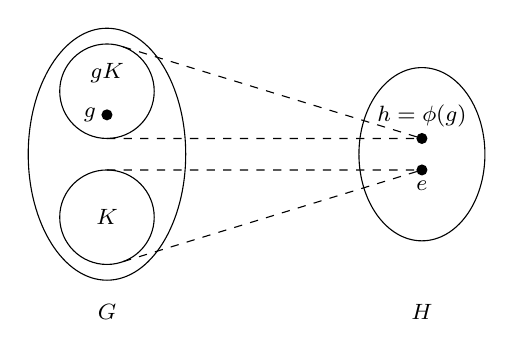
\begin{tikzpicture}
            \footnotesize
            \draw
                (-2,0) ellipse (1cm and 1.6cm)
                (2,0) ellipse (0.8cm and 1.1cm)
            ;
            \node at (-2,-2) {$G$};
            \node at (2,-2) {$H$};
    
            \draw
                (-2,0.8) circle (6mm) node[above]{$gK$}
                (-2,-0.8) circle (6mm) node{$K$}
            ;
            \fill
                (-2,0.5) circle (2pt) node[left=1pt]{$g$}
                (2,0.2) circle (2pt) node[above=1pt]{$h=\phi(g)$}
                (2,-0.2) circle (2pt) node[below=1pt]{$e$}
            ;
            \draw [dashed]
                (-2,0.2) -- (2,0.2)
                (-2,0.8) ++(70:0.6) -- (2,0.2)
                (-2,-0.2) -- (2,-0.2)
                (-2,-0.8) ++(-70:0.6) -- (2,-0.2)
            ;
        \end{tikzpicture}
        \caption{Visualizing a surjective homomorphism.}
        \label{fig:surjHom}
    \end{figure}
    \begin{itemize}
        \item In general, we know that $K\mapsto\{e\}$.
        \item Since $\phi$ is surjective, every $h\in H$ equals $\phi(g)$ for some $g\in G$.
        \item More broadly, $gK\mapsto\{h\}$.
        \item Can you get more elements than those in $gK$ that map to $h$? Perhaps elements of $Kg$ or $KgK$? Well since $K$ is normal, $kg=gk$.
        \item Thus, all surjective homomorphisms have the same general structure.
        \begin{itemize}
            \item In particular, they all map disjoint cosets to single elements.
            \item Alternatively, we can take the perspective that they send every element to their coset with the kernel.
        \end{itemize}
    \end{itemize}
    \item Lemma: If $\phi:G\to H$ is a surjective homomorphism, $h\in H$, $\phi(g)=h$, and $K=\ker\phi$, then $\phi^{-1}(h)=gK$.
    \begin{proof}
        % , $\phi(g')=h=\phi(g)$ where $x\in G$, $g'=gx$, $\phi(g')=\phi(g)\phi(x)$, and $e=\phi(x)$, as desired.
        
        % Then $\phi(g')=\phi(g)\phi(x)$, but since $\phi


        Suppose $g'\in\phi^{-1}(h)$. Suppose $g'=gx$ (we do know that such an $x$ exists in $G$; in particular, choose $x=g^{-1}g'$). Then
        \begin{equation*}
            \phi(g') = \phi(gx)
            = \phi(g)\phi(x)
        \end{equation*}
        Since $\phi(g')=h=\phi(g)$, we have by the cancellation lemma that
        \begin{equation*}
            e = \phi(x)
        \end{equation*}
        i.e., $x\in K$. Therefore, $g'\in gK$, as desired.
    \end{proof}
    \item We can define a bijection $\tilde{\phi}:G/K\mapsto H$ defined by $gK\mapsto\phi(g)$.
    \item Claim: $\tilde{\phi}$ is an isomorphism of groups.
    \begin{proof}
        Need to check that $\tilde{\phi}$ is a homomorphism, surjective, and injective. We also need to check that it is well-defined (we did this with our picture).\par
        Surjective: Let $h\in H$ be arbitrary. Then $h=\phi(g)$. It follows that $h=\tilde{\phi}(gK)$.\par
        Injective: Show that $\ker\tilde{\phi}=\{eK\}$. Let $gK\in\ker\tilde{\phi}$. Then $\phi(g)=\tilde{\phi}(gK)=e$. Thus, $g\in K$. Therefore, $gK=eK$, as desired.\par
        Homomorphism: Check $\tilde{\phi}(xK)\tilde{\phi}(yK)=\tilde{\phi}(xyK)$. Since $\tilde{\phi}(zK)=\phi(z)$, we have the desired property. Explicitly,
        \begin{equation*}
            \tilde{\phi}(xyK) = \phi(xy)
            = \phi(x)\phi(y)
            = \tilde{\phi}(xK)\tilde{\phi}(yK)
        \end{equation*}
    \end{proof}
    \item Takeaway: All surjective homomorphisms are somewhat the same.
    \item Generalize:
    \item Let $\phi:G\to H$ be a homomorphism.
    \begin{itemize}
        \item We know that $G\twoheadrightarrow\im\phi\hookrightarrow H$. Essentially, we can break up any homomorphism into the composition of a surjective homomorphism onto the image and an injective homomorphism into $H$.
    \end{itemize}
    \item Theorem (FIT: First Isomorphism Theorem): To every homomorphism $\phi$ there corresponds an isomorphism $\tilde{\phi}:G/\ker\phi\to\im\phi$ such that
    \begin{equation*}
        \tilde{\phi}(g\cdot\ker\phi) = \phi(g)
    \end{equation*}
    \begin{figure}[h!]
        \centering
        \begin{tikzpicture}[
            node distance=3mm,
            text height=1.5ex,text depth=0.25ex
        ]
            \small
            \node (G) at (150:1) {$G$};
            \node (Gk) at (-90:1) {$G/\ker\phi$};
            \node (Gi) at (30:1) {$\im\phi$};
            \node (H) at ([xshift=1.73cm]30:1) {$H$};
            
            \footnotesize
            \draw [->>] (G) -- (Gk);
            \draw [->] (Gk) -- node[above,sloped]{$\sim$} node[below right,yshift=3pt]{$\tilde{\phi}$} (Gi);
            \draw [->>] (G) -- node[above]{$\phi$} (Gi);
            \draw [right hook->] (Gi) -- (H);
    
            \node (g1) [above=of G] {$g$};
            \node (g2) [left=of G] {$g$};
            \node (gk) [node distance=7mm,below=of Gk] {$g\cdot\ker\phi$};
            \node (gi1) [above=of Gi] {$\phi(g)$};
            \node (gi2) [below right=of Gi,xshift=-6mm,yshift=2mm] {$\phi(g)$};
    
            \draw [|->] (g1) -- (gi1);
            \draw [|->] (g2) -- (gk);
            \draw [|->] (gk) -- (gi2);
    
            \path (-3,0) -- (3,0);
        \end{tikzpicture}
        \caption{First isomorphism theorem.}
        \label{fig:isoTrm1}
    \end{figure}
    \begin{itemize}
        \item The triangle is \textbf{commutative}. This means that sending $g$ along both paths gets you to the same result.
        \item The way to understand normal subgroups is to understand the homomorphisms.
    \end{itemize}
    \item $N\subset G$ is normal if
    \begin{enumerate}
        \item $N$ is a subgroup.
        \item $N$ is normal, i.e., $N$ is a union of conjugacy classes.
        \item $e\in N$.
        \item $|h|\big||G|$ (Lagrange).
    \end{enumerate}
    \item 3-4 both follow from 1. They are not sufficient conditions for normality, but they can put restrictions on what is normal and make the computation easier.
    \item Examples.
    \begin{itemize}
        \item Let $\phi:\Z\to H$ send $1\mapsto h$ and $k\mapsto h^k$ (see Figure \ref{fig:FITexample}).
        \begin{figure}[h!]
            \centering
            \begin{tikzpicture}[
                node distance=3mm,
                text height=1.5ex,text depth=0.25ex
            ]
                \small
                \node (Z) at (135:1) {$\Z$};
                \node (ZnZ) at (-135:1) {$\Z/n\Z$};
                \node (h) at (-45:1) {$\gen{h}$};
                \node (H) at (45:1) {$H$};
                
                \footnotesize
                \draw [->>] (Z) -- (ZnZ);
                \draw [->] (ZnZ) -- node[above]{$\sim$} (h);
                \draw [right hook->] (h) -- (H);
                \draw [->] (Z) -- (H);
        
                \node (kpnZ) [below=of ZnZ] {$k+n\Z$};
                \node (hk) [below=of h] {$h^k$};
        
                \draw [|->] (kpnZ) -- (hk);
            \end{tikzpicture}
            \caption{An example of the FIT.}
            \label{fig:FITexample}
        \end{figure}
        \begin{itemize}
            \item $\im\phi=\gen{h}$.
            \item $\ker\phi=n\Z$ where $|h|=n$; if $|h|=\infty$, then $\ker\phi=\{0\}$.
            \item The FIT tells us that there is a map from $\Z$ to $\Z/n\Z$ to $\gen{h}$ to $H$. The first map sends $k\mapsto k+n\Z$ and the second sends $k+n\Z\mapsto h^k$.
        \end{itemize}
        \item Let $G=S_3$.
        \begin{itemize}
            \item The conjugacy classes are
            \begin{align*}
                \{e\}&&
                \{(1,2),(1,3),(2,3)\}&&
                \{(1,2,3),(1,3,2)\}
            \end{align*}
            \item Thus, the only possible normal subgroup $N$ is
            \begin{equation*}
                H = \{e\}\cup(xxx)
                = \gen{(1,2,3)}
            \end{equation*}
            \begin{itemize}
                \item $e\in N$ eliminates union 2,3; Lagrange eliminates union 1,2 (which has order 4).
            \end{itemize}
        \end{itemize}
        \item Let $G=S_4$.
        \begin{itemize}
            \item The conjugacy classes are
            \begin{align*}
                e&&
                (xx)&&
                (xxx)&&
                (xxxx)&&
                (xx)(xx)
            \end{align*}
            \item The number of elements of the above form is
            \begin{align*}
                1&&
                6&&
                8&&
                6&&
                3
            \end{align*}
            \item The divisors of $|S_4|=24$ are 1,2,3,4,6,8,12,24.
            \begin{itemize}
                \item 1 is possible; no way to get 2,3; 4 is possible; 6,8 are impossible; 12,24 are possible.
                \item The 4 example is
                \begin{equation*}
                    K = \gen{e,(1,2)(3,4),(1,3)(2,4),(1,4)(2,3)}
                \end{equation*}
            \end{itemize}
        \end{itemize}
    \end{itemize}
    \item $S_3/\gen{(1,2,3)}\cong\Z/2\Z$.
    \item $S_4/K$ is a group of order 6.
    \item The first instance corresponds to some map from $S_3\to S_2$.
    \begin{itemize}
        \item You can get an isomorphism from $S_3$ to $D_6$.
        \item The surjective map sends rotations to the identity and reflections to the nonidentity element.
        \item By the FIT, $S_3/\gen{(1,2,3)}\cong S_2$.
        \begin{itemize}
            \item Yes, if you know enough about the quotient group, you can think about its properties. But it's easier to use the FIT.
        \end{itemize}
    \end{itemize}
    \item We constructed a map $S_4\to\text{Cu}\to S_3$. If $N=\ker$, by the FIT, $S_4/N\cong S_3$.
    \begin{itemize}
        \item As per the above example, we need to take $N=K$ here.
    \end{itemize}
    \item Example: $G=\text{O}(2)$.
    \begin{itemize}
        \item The normal subgroups of $\text{O}(2)$ are $\{e\}$, $\{r,r^{-1}\}$, and $\{\text{reflections}\}$.
        \item If $N\triangleleft\text{O}(2)$ contains a reflection, then $N=\text{O}(2)$.
        \item Let $N\subset\text{SO}(2)$ be such that $|N|=k$, i.e., $N$ is generated by the rotation of $2\pi k/N$. What is $\text{O}(2)/N$? You can think of $\text{SO}(2)$ as a rotation in $\R$. Thus, $\R/2\pi\Z\cong\text{O}(2)$. Thus, $\text{SO}(2)/N\cong\text{SO}(2)$.
    \end{itemize}
    \item Next time: Replace $S_4$ with $S_5$.
    \item The midterm is most likely Wednesday next week.
    \begin{itemize}
        \item The midterm will not be on Monday, but it could test stuff covered next Monday.
    \end{itemize}
    \item Read the blog post on dihedral groups and the other blog posts I've missed!
\end{itemize}



\section{Blog Post: The First Isomorphism Theorem}
\emph{From \textcite{bib:Calegari}.}
\begin{itemize}
    \item \marginnote{11/12:}Again, a fairly straight review of class.
    \item Implication of the FIT: The image of \emph{any} homomorphism $\phi$ is naturally (i.e., isomorphic to) the quotient group of $G/\ker\phi$.
    \item A direct statement and proof of the FIT is given.
    \item Example: We can use the FIT to prove that $S_4/K\cong S_3$, which would be painful to verify by hand.
    \item "First" Isomorphism Theorem?
    \begin{itemize}
        \item There are other isomorphism theorems, but since they are all consequences of the first, Calegari recommends we only memorize the first.
    \end{itemize}
    \item Theorem (Second Isomorphism Theorem): Let $G$ be a group, $H$ a subgroup, and $N$ a normal subgroup of $G$. Then there is an isomorphism
    \begin{equation*}
        H/(H\cap N) \cong HN/N
    \end{equation*}
    \item What this means:
    \begin{itemize}
        \item $HN=\{hn\mid h\in H,\ n\in N\}$.
        \item $HN$ is a subgroup of $G$ since
        \begin{equation*}
            (hn)_1(hn)_2 = h_1n_1h_2n_2
            = h_1(h_2h_2^{-1})n_1h_2n_2
            = \underbrace{h_1h_2}_{\in H}\underbrace{(h_2^{-1}n_1h_2)n_2}_{\in N}
        \end{equation*}
        \item Since $e\in H$, $N\subset HN$. Moreover, $N\triangleleft HN$ since $N\triangleleft G$.
        \item $H\cap N$ is normal in $H$: If $n\in H\cap N$ and $h\in H$, then $hnh^{-1}\in N$ since $N\triangleleft G$; $hnh^{-1}\in H$ since $n,h\in H$; and therefore, $hnh^{-1}\in H\cap N$.
    \end{itemize}
    \item If we now define a map $\phi(h(H\cap N))=hN$, we can easily prove that it is well-defined, surjective, injective, and a homomorphism.
    \item Calegari can't really think of any applications of the SIT, so he recommends we forget it and just view the proof as another exercise in thinking about the constructions we introduced in building up to the FIT.
    \item Why normal subgroups are interesting:
    \begin{itemize}
        \item The FIT asserts that any homomorphism of groups $\phi:G\to H$ can be understood by understanding (1) the subgroups of $H$ (one of which will be $\im\phi$) and (2) the quotients $G/K$ of $G$.
        \item These problems can be studied individually.
        \item Thus, to understand maps among the $S_n$ for example which we're often interested in, we should study these two things.
    \end{itemize}
    \item Union of conjugacy classes and $e\in N$ / Lagrange lemma.
\end{itemize}



\section{The Alternating Group}
\begin{itemize}
    \item \marginnote{10/21:}Today, we continue our investigation of normal subgroups.
    \item Recall our conditions for normal subgroups that we can check first as constraints before doing the formal evaluation.
    \item Normal subgroups of $S_5$.
    \begin{table}[H]
        \centering
        \begin{tabular}{l|c|c}
            $(x)$ & 1 & $\subset H$\\
            $(xx)$ & 10 & X\\
            $(xxx)$ & 20 & \\
            $(xxxx)$ & 30 & X\\
            $(xxxxx)$ & 24 & $\subset H$\\
            $(xx)(xx)$ & 15 & $\subset H$\\
            $(xx)(xxx)$ & 20 & \\
        \end{tabular}
        \caption{Counting $S_5$ cycle decompositions.}
        \label{tab:normalS5}
    \end{table}
    \begin{itemize}
        \item $H=\{e\},S_5$ are normal subgroups.
        \item $|H|=11$. Nope.
        \item $|H|=16$. Nope.
        \item Let's change strategy: Divisors of 120 that are greater than 16 are 120, 60, 40, 30, 24, and 20.
        \item Can't hit 20, 24, 30.
        \item Possibility 1: $H=\{e\}\cup\{(xx)(xx)\}\cup\{(xxxxx)\}$.
        \item We know that the $\subset H$ subgroups must be included if we want to get a multiple of 10 greater than 40.
        \item Possibility 2: $H=\{e\}\cup\{(xx)(xx)\}\cup\{(xxxxx)\}\cup\{(xxx)\}$.
        \item Possibility 3: $H=\{e\}\cup\{(xx)(xx)\}\cup\{(xxxxx)\}\cup\{(xxx)(xx)\}$.
        \item Which of these, if any, are subgroups of $S_5$?
        \item We know that the X'ed out subgroups cannot be included because they generate $S_5$.
        \item $n$-cycles imply 3-cycles since
        \begin{equation*}
            (n,n-1,\dots,4,2,3,1)\cdot(1,2,3,4,\dots,n) = (1,3,2)
        \end{equation*}
        \item Thus, we lose 1 and 3.
        \item It follows that if $H\triangleleft S_5$ is proper and nontrivial, then $|H|=60$ and $H$ equals possibility 2, or there is no such $H$.
        \item We now show that possibility 2 is a group and apply a construction more general than technically necessary but it will be useful later.
        \item We've already seen possibility 2: It's the symmetries of the dodecahedron $D_0\subset S_5$ from the homework.
        \item Thus, the only proper subgroup of $S_5$ is this one (which we will later equate to a group called $A_5$).
    \end{itemize}
    \item \textbf{Alternating} (group of order $n$): The set of all $g\in S_n$ that can be written as the product of an even number of transpositions. \emph{Denoted by} $\bm{A_n}$.
    \item $A_n$ is a subgroup:
    \begin{itemize}
        \item $e=\tau\tau^{-1}$.
        \item Product of an even number of 2-cycles: Add an even number of 2 cycles to an even number of 2-cycles; still have an even number.
        \item Inverse is same length: $\sigma=\tau_1\cdots\tau_{2k}$; $\sigma^{-1}=\tau_{2k}^{-1}\cdots\tau_1^{-1}$.
    \end{itemize}
    \item Proposition: Either $A_n$ is normal of index 2, $|A_n|=n!/2$, or $A_n=S_n$.
    \item Claim: Let $\sigma\in S_n\setminus A_n$ be such that $\sigma=\tau_1\cdots\tau_{2k+1}$. Then $S_n=A_n\cup\sigma A_n$.
    \begin{proof}
        Let $g\in S_n$ be arbitrary. We divide into two cases. If $g$ is the product of an even number of transpositions, then $g\in A_n$. If $g$ is the product of an odd number of transpositions, then $\sigma^{-1}g$ is the product of an even number of transpositions, i.e., $g\sigma^{-1}\in A_n$. But this implies that $g\in\sigma A_n$, as desired.
    \end{proof}
    \item Define $C_n$ to be the set of all $g\in S_n$ that is a product of a multiple of three 2-cycles. This is just equal to $S_n$ because $(a,b)=(a,b)(a,b)(a,b)$, so it contains all 2-cycles, so it generates $S_n$.
    \item So we want to prove that $A_n$ preserves a property (some invariant) that general elements of the symmetric group of not.
    \item Let $n\geq 2$. There are $\binom{n}{2}$ pairs $\{i,j\}$ in $[n]$. We now take the product of all ordered pairs, or all ordered pairs where $i>j$. This is equal to 1 if $\sigma(i)>\sigma(j)$ and equal to $-1$ if $\sigma(i)<\sigma(j)$. All 2-cycles swap an odd number of things around. We can thus take
    \begin{equation*}
        \prod_{i>j}\frac{\sigma(i)-\sigma(j)}{i-j}
    \end{equation*}
    \begin{itemize}
        \item This leads to an argument, but we wanna give a slick argument.
    \end{itemize}
    \item Here's a trick that's a bit subtle.
    \item Work in $\R^n$; think about the standard basis of orthonormal vectors. Represent $S_n$ as a subset of $O(n)$ (the subset of all permutation matrices with one 1 in every row and column and zeroes everywhere else) and then compose it with the determinant map to get to $\pm 1$. This is a homomorphism. It sends all 2-cycles to $-1$. So the things that are all products of an even number of 2-cycles, we send to 1. Check \textcite{bib:DummitFoote} for more details.
    \item Theorem: Assume $n\geq 2$.
    \begin{enumerate}
        \item $A_n$ is generated by 3-cycles.
        \item $A_n$ is generated by $k$-cycles where $k$ is odd.
        \item If $n\geq 5$, then the only proper normal subgroup of $S_n$ is $A_n$.
    \end{enumerate}
    \begin{proof}
        $1\Rightarrow 2$: If $k\geq 3$ and odd, take
        \begin{equation*}
            (k,\dots,2,3,1)(1,2,\dots,k) = (1,3,2)
        \end{equation*}
        Note: $(1,\dots,k)=(1,2)(1,3)\cdots(1,k)$.\par
        1: $A_n$ is generated by all products of two 2-cycles. Three cases:
        \begin{align*}
            (a,b)(c,d) &= (c,a,d)(a,b,c)\\
            (a,b)(a,c) &= (a,c,b)\\
            (a,b)(a,b) &= e
        \end{align*}
        3: We want $H\triangleleft S_n$. We know that if $(xxx)\in H$, then $A_n\triangleleft H$.\par
        Case 1: $\sigma\in H$ with $\sigma=(xxx\cdots x)(xx)(xxx)\dots$ (i.e., at least one component $k$-cycle satisfies $k\geq 3$). Implies that we can generate a three cycle by the $n$-cycles implies 3-cycles approach.\par
        Case 2: $\sigma=(xx)(xx)\cdots(xx)$ ($\sigma$ is a product of disjoint two cycles; "the only thing left" after case 1). Subcase 0: $\sigma=(ab)$. Implies $H=S_n$. Subcase 1: $\sigma=(ab)(cd)$. Multiply by $(a,b)(c,e)$ to get $(c,e,d)$. Subcase 2: $\sigma=(a,b)(c,d)(e,f)\cdots$. Choose $(a,c)(b,e)(d,f)$. Then $(a,b)(c,d)(e,f)\cdot(a,c)(b,e)(d,f)=(a,d,e)(b,f,c)$. We've reduced to the previous case at this point, i.e., we can now get it to $(a,d,e)$.
    \end{proof}
    \item Misc. notes:
    \begin{itemize}
        \item When you have two things, you need that extra space of an $e$. If $n=4$ it's false because there are other normal subgroups. Note that $S_3$ actually does work in this proof; it's just $n=4$ that causes the issue.
    \end{itemize}
    \item Corollary: Let $n\geq 5$. Let $\phi:S_n\to\Gamma$ be a homomorphism. Then 3 possible things occur.
    \begin{enumerate}
        \item $\im\phi=\{e\}$.
        \item $\im\phi\cong\Z/2\Z$.
        \item $\im\phi\cong S_n$.
    \end{enumerate}
    \begin{proof}
        By the FIT, $\im\phi\cong S_n/\ker\phi$. Since $\ker\phi\triangleleft S_n$, we have that $\ker\phi=S_n$, $\ker\phi=A_n$, or $\ker\phi=\{e\}$. These three cases correspond to possibilities 1-3, respectively.
    \end{proof}
    \item This does imply the surjective homomorphism thing.
    \item Notes on the exam: The material in this class covered on Monday may be tested. Emphasis on it not being too long. He will not be able to avoid one "fun" small amount of credit problem. Look at the practice problems! Would not be as hard as the riffle shuffle problem. A boring problem is "do a computation" or "is it a subgroup? No: It violates Lagrange's theorem." A fun problem is more like some of the practice/HW problems.
\end{itemize}




\end{document}